\scanpage{4}
\mspage{2}
on $\mathcal E^{(\nu)}$ a graded \deleted{algebra}\inserted{ring} structure ?

It suffices that we have the relations $(1.1)$
\[
\deleted{\unsure{*}}\quad\left\{\begin{aligned}
\pi_i^2&=\pi_i\\
\pi_i\pi_j&=\pi_j\pi_i=0\quad\text{if }i\neq j\\
\sum\pi_i&=1
\end{aligned}\right.
\]
which imply that the $\operatorname{pr}_{\nu}^{\mathcal E}$ defined by $(1.2.)$ are pairwise orthogonal projections with sum $1$, hence that the $\mathcal E^{(\nu)}$ do indeed define a grading \inserted{\figure{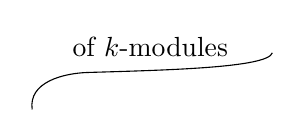
\begin{tikzpicture}[x=1cm,y=1cm]\node at (0,.35) {of $k$-modules};\draw (-1.5,-.45) .. controls (-1.55,-.1) and (-1.1,.01) .. (-.8,.02) .. controls (.2,.05) and (1.5,.08) .. (1.55,.27);\end{tikzpicture}}} on $\mathcal E^{(\nu)}$, \deleted{then}\inserted{and} that
\[
\mathcal E^{(\nu)}\mathcal E^{(\nu')}\subset\mathcal E^{(\nu-\nu')}.
\]
\margin{one can replace $\mathbb Z$ by an arbitrary \unsure{\uline{abelian}\ group|\uline{group}|\uline{group}}}
Note also that $(1.4.)$ that $(1.4)$ are valid, for \deleted{we also have the decomposition}
\[
\deleted{u=\sum_{ij}\pi_j u\pi_i}
\]
\deleted{whence the relation}
\[
\deleted{\pi_{i+\nu}u\pi_i=\unsure{\pi_\nu|\pi_j|\pi_{i+\nu}}u\pi_i}
\qquad\inserted{\mathcal E_i^j}
\]
\[
\left\{\begin{aligned}
\mathcal E&=\bigoplus_{i,j}\pi_j\mathcal E\pi_i\\
\operatorname{pr}_{i,j}(u)&=\pi_j u\pi_i
\end{aligned}\right.
\qquad\text{hence }u=\sum_{\alpha,\beta}\pi_\beta u\pi_\alpha
\]
and the relation $u\pi_i=\pi_{i+\nu}u$ implies, since
\[
u\pi_i=\sum_\beta\pi_\beta u\pi_i,\quad\text{and}\quad
\pi_{j+\nu}u=\sum_i\pi_{j+\nu}u\pi_\alpha,
\]
that
\[
\pi_\beta u\pi_i=0\quad\text{if }\beta\neq i+\nu.
\]
\margin{\figure{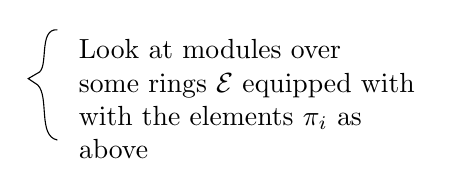
\begin{tikzpicture}[x=1cm,y=1cm]
\node[anchor=north west,align=left] at (.4,1.4) {Look at modules over\\\deleted{some} rings $\mathcal E$ equipped \deleted{with}\\with the elements $\pi_i$ as\\above};
\draw (.25,1.4) .. controls (0,1.42) and (.15,.9) .. (0,.85) --(-.12,.78) --(0,.7) .. controls (.15,.55) and (0,.05) .. (.25,0);
\end{tikzpicture}}}

3. \deleted{We want} Let us finally start from a graded \deleted{algebra}\inserted{ring} $\mathcal E^*$ \deleted{over $k$}, and let us ask ourselves the question of the existence and \uline{the uniqueness} of a family $(\pi_i)_{i\in\mathbb Z}$ of elements of $\mathcal E^*$, \inserted{\figure{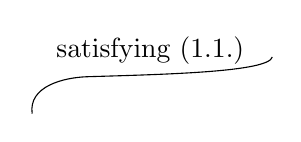
\begin{tikzpicture}[x=1cm,y=1cm]\node at (0,.35) {satisfying $(1.1.)$};\draw (-1.5,-.45) .. controls (-1.55,-.1) and (-1.1,.01) .. (-.8,.02) .. controls (.2,.05) and (1.5,.08) .. (1.55,.27);\end{tikzpicture}}} defining the grading, by $(1.3.)$ (hence by $(1.4)$). We \deleted{suppose} suppose here that
\mspage{3}
